\section{Einleitung}
\subsection{Theoretische Grundlagen}
\subsubsection{Moderne Lawinenkunde}
Lawinenprobleme lassen sich grundsätzlich aus zwei Perspektiven betrachten und vorhersagen: Einerseits auf Basis der Schneedecke, anderer seits auf Basis von Geländeformen und Statistik.
Dabei wird bei der praktischen Lawinenkunde auf das erstellen von beispielsweise Schneeprofilen (Extended Coloumn Test) zur Einschätzung der lokalen Stabilität der Schneedecke gesetzt.

Bei der analytischen Lawinenkunde arbeiten wir mit historischen Unfalldaten, konkret ist das Ziel, ein qunatitatives Mass für das eingegangene Riskio zu errechnen.
Wir korrelieren also bekannte konsequenzen mit der Hangform und deren Eintrittswahrscheinlichkeit. Es folgt also unser Risikobegriff:
\begin{equation}
  r = k \cdot \frac{u}{b}
\end{equation}
wobei $r$ unser Risiko darstellt, $u$ die Anzahl Unfälle und $b$ die Anzahl Begehungen.
Anders ausgedrückt, misst das Risiko nicht in welchem Anteil der Begehungen ein Unfall eintritt, sondern, wie gross ein eintretender Unfall statistisch sein wird.

Dies steht der praktischen Lawinenkunde gegenüber. Hier beobachten wir die Schneedecke und leiten daraus die Entscheidung ab, weiter aufzusteigen oder umzukehren – diese Entscheidung steht in beiden Gebieten im Vordergrund.
\columnbreak
\subsubsection{Schema 3x3}
Der Goldstandard der Tourenplanung ist heute Werner Munters 3x3-Schema. Dabei werden in drei <<Zoom>>-Stufen drei Faktoren ausgewertet:
\vfill
\textbf{Regional} 
Von zuhause aus \cite{munter}:
\begin{itemize}
  \item Verhältnisse: 1. Lawinenlagebericht LLB, 2. Wetterprognose, 3. Auskünfte von Einheimischen/Hüttenwart
  \item Gelände: 1. $1:25000$-Karte, 2. Tourenführer, 3. Eigene Geländekentnisse
  \item Menschen: 1. Wer ist Dabei?, 2. Ausbildung, 3. Material, 4. Emotionale und Phyische Kondition? 
\end{itemize}

\textbf{Lokal} Im Gebiet, soweit die Sicht reicht \cite{munter}\cite{redbull3x3}:
\begin{itemize}
  \item Verhältnisse / Schneedecke / Wetter: 1. Sicht?, 2. Bewölkung, Wind, Niederschlag, Temperatur?, 3. Schneeverfrachtungen, Neuschneemenge, 4. Stimmt der LLB?
  \item Gelände: 1. Stimmt meine Vorstellung (Steilheit, Exposition)? 2. Spuren anderer Gruppen
  \item Menschen: 1. Ausrüstungskontrolle (Gruppencheck LVS), 2. Andere Gruppen unterwegs?
\end{itemize}
\textbf{Zonal} Im Einzelhang \cite{munter}\cite{redbull3x3}:
\begin{itemize}
  \item Verhältnisse: 1. Neuschneemenge, 2. Triebschnee, 3. Mögliche Abrisszonen, 4. Sonneneinstrahlung
  \item Gelände: 1. Wer / was ist über/unter der Gruppe?, 2. Steilste Stelle?, 3. Exposition, 4. Typisches Lawinengelände, 5. Hangform, 6. Höhe, 7. Oft befahren?
  \item Menschen: 1. Können \& Kondition, 2. Vorischtsmassnahmen, 3. Sichere Sammelstellen
\end{itemize}

\vfill
\subsubsection{Digitale Höhenmodelle}

In den 1960er Jahren verlangte der schweizer Generalstab vom heutigen Bundesamt für Landestopografie zu prüfen, ob tief fliegende feindliche Kampfflugzeuge unbemerkt in die Schweiz eindringen konnten. Um die für diese Prüfung nötigen Berechnungen erstmals an einem Grossrechner ausführen zu können, mussten die topographischen Höhen aus der Landeskarte $1:250000$ auf Lochkarten transferiert werden. Mit einer Auflöung von \qty{250}{m} wurden die Höhenlinien der analogen Kartenprodukte so in mühseliger Handarbeit zwischen 1966 -- 1968 erstmals digital nutzbar gemacht. Das so erstellte digitale Höhenmodel DEM <<RIMINI>> wurde bis in die 1970er Jahre genutzt. \cite{swisstopohistdem}

Rufe nach einem engmaschigerem Modell brachten schliesslich unter anderem <<DHM25>> hervor, welches eine Auflösung von bereits \qty{25}{m} mitbringt. \cite{swisstopohistdem}

Um die Jahrtausendwende erfolgte dank schnelleren CPUs und günstigem Datenspeicher eine Umkehrung des Prozess. Neu werden die analogen Landeskarten auf Basis eines DEM erstellt. Moderne DEMs erreichen dabei eine Auflösung bis zu \qty{0.5}{m} bei einer Genauigkeit von 0.5 -- 3 \unit{m} \cite{alti3dprod}. SwissAlti\textsuperscript{3D} ist genau ein solches Modell.

Dank der <<Open Government Data Strategie>> des Bundes werden seit 2020 diverse Datensammlungen die öffentliche Verwaltungen produzieren der Öffentlichkeit zur Verfügung gestellt \cite{opendataswiss}.
So landet nebst dem Fahrplan der SBB, Jungwaldflächen und den Standorten aller öffentlichen Toiletten der Stadt Luzern auch  SwissAlti\textsuperscript{3D} auf dem Opendataprotal des Bundes.

SwissAlti\textsuperscript{3D} wird als GeoTIFF ausgeliefert. GeoTIFF sind letztendlich nur Bilddaten, die um einen Eintrag zur Lokalisierung in einem Koordinatensystem, hier LV95 LN02, ergänzt wurden. Der Farbwert eines Pixel entspricht jedoch der Höhe an dieser Stelle. Insgesamt wird die Schweiz in ca. $43500$ $\qty{1}{km} \times \qty{1}{km}$ grosse Kacheln unterteilt. \cite{alti3dprod}

\subsubsection{Relevante Geländefaktoren}

\subsubsection{Unfalldaten \& Begehungen}


\subsection{Methodik}
\subsubsection{Berechnung von topographischen Oberflächenfaktoren}

Wir schneiden $3 \times 3$-Ausschnitt aus dem Höhenmodell. Unser Ziel ist es, die chrakteristischen Geländeeigenschaften für die Zelle $e$ zu berechen.
$a$ -- $h$ sind die Höhen an einem bestimmten Gitterpunkt:

\begin{Figure}
  \centering
  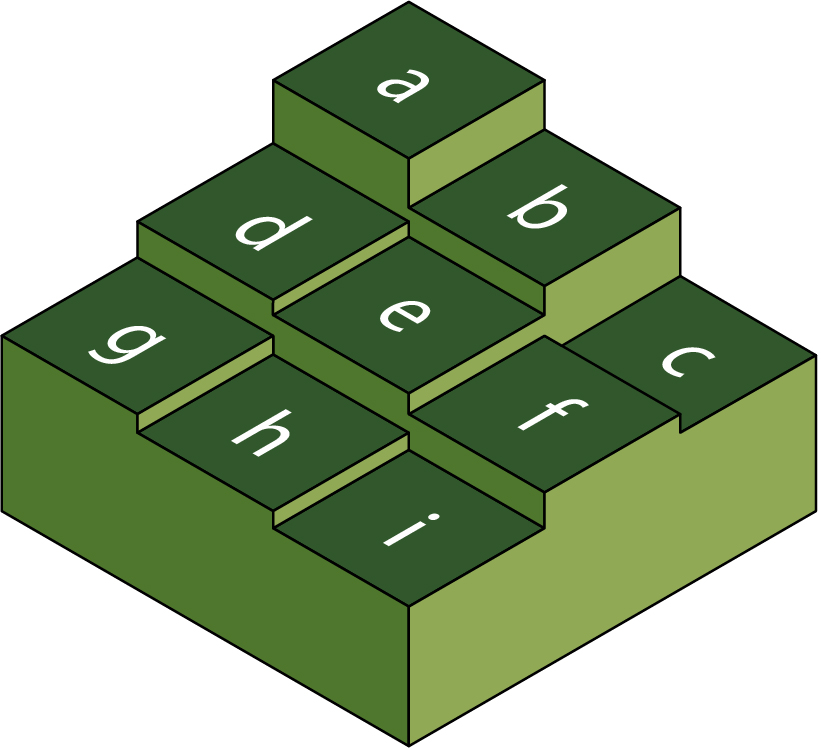
\includegraphics[width=5cm]{isoGrid}
  \captionof{figure}{$3 \times 3$-Ausschnitt von Höhen aus einem DEM und deren Benennung}
\end{Figure}

Hangneigung und Exposition nach \cite{gisslopeaspect}:

\begin{equation} \label{eq1}
  \frac{\Delta z}{\Delta x} = \frac{(c + 2f + i) - (a + 2d + g)}{8r}
\end{equation}
\begin{equation} \label{eq2}
  \frac{\Delta z}{\Delta y} = \frac{(g + 2h + i) - (a + 2b + c)}{8r}
\end{equation}

Hangneigung $\rho$ und Exposition $\theta$:
\begin{align}
  \rho &= \arctan \left( \sqrt{
    \left( \frac{\Delta z}{\Delta x}\right)^2 + 
    \left(\frac{\Delta z}{\Delta y}\right)^2}
  \right)\\
  \theta &= \arctan\left(\frac{\frac{\Delta z}{\Delta x}}{-\frac{\Delta z}{\Delta y}}\right)
\end{align}

Geländekrümmung nach \cite{gismath}:
\begin{align}
  D &= \frac{{(d + f) / 2 - e}}{{r^2}} \\
  E &= \frac{{(b + h) / 2 - e}}{{r^2}} \\
  F &= \frac{{-a + c + g - i}}{{4r^2}} \\
  G &= \frac{{-d + f}}{{2r}} \\
  H &= \frac{{b - h}}{{2r}}
\end{align}

(6) -- (10) sind die Faktoren eines teilweisen Polynom vierten Grades \cite{gismath}.
Hangkrümmung $c_{Plan}$ und $c_{Profil}$ beschreiben, mit welchem Radius sich die Hangneigung parallel (Plankrümmung) bzw. senkrecht (Profilkrümmung) zur Exposition ändert:

\begin{align}
    c_{Plan} &= -\frac{{2(DH^2 + EG^2 - FGH)}}{{G^2 + H^2}}
    \\
    c_{Profil} &= \frac{{2(DG^2 + EH^2 + FGH)}}{{G^2 + H^2}}
\end{align}



\subsubsection{Parallele Berechnungen}
\subsubsection{Rechenleistung zur freien Verfügung}
\subsubsection{3D-Karte im Webbrowser}